%% ------------------------------------------------------------------------------------------- Dataset
\section{Dataset}
\label{sec:data}

\noindent\textbf{Source and labels.} HaGRIDv2~\cite{hagridv2} (CC BY-SA 4.0 variant) has 1.08M FullHD images of
consenting subjects. Each image has gesture boxes and labels, a \texttt{user\_id}, and \emph{automatically
estimated} age, gender and race. We use HaGRID's \emph{official subject-disjoint} split and the gesture classes
like, peace, palm, fist, ok and one. MediaPipe is scored on the 5 of them it supports. The archives are 40\,GB per
class, so \texttt{fetch\_hagrid.py} reads the ZIP central directories with HTTP range requests and downloads only
the selected images ($\approx$1.2\,GB, 2\,min).

\noindent\textbf{Split and size.} \emph{Test}: 603 test subjects show all six gestures. We draw 100 of them at
random (seed 441) and take one image per (subject, gesture). This gives \textbf{600 images at native resolution}
(mostly 1440$\times$1920; 60\% of images female, 80\% annotated White). \emph{Val}: 50 images per class, each from
a different val subject (300). The val set is used only to choose the ROI settings. The image ids are stored in
\texttt{selection.json}. No test subject appears in val.

\noindent\textbf{Test conditions (our construction).}
The proposal planned a volunteer set captured in a classroom, which we did not collect (\cref{sec:fail}).
Instead, \texttt{make\_conditions.py} derives four conditions from each source image. Each output is a
deterministic function of (image, condition, seed), so the baseline and ours see identical inputs (\cref{fig:cond}).
\emph{normal}: unchanged.
\emph{low light}: brightness $\times$0.35, gamma 1.4, Gaussian noise $\sigma{=}6$, JPEG q85.
\emph{far}: the image is pasted at native resolution into the centre of a canvas twice as wide and twice as tall, so the subject covers $\frac{1}{4}$ of the frame.
\emph{crowded}: a \emph{different} subject showing a \emph{different} gesture is pasted at 0.6$\times$ scale
beside the claimant. This doubles as the \emph{background-hand attack}: if the challenge is the other person's
gesture, a correct system must reject.
The result is 2,400 test images (2,000 with MediaPipe's 5 gestures) and, from the val images, a 1,200-image val set.

\begin{figure}[t]
  \centering
  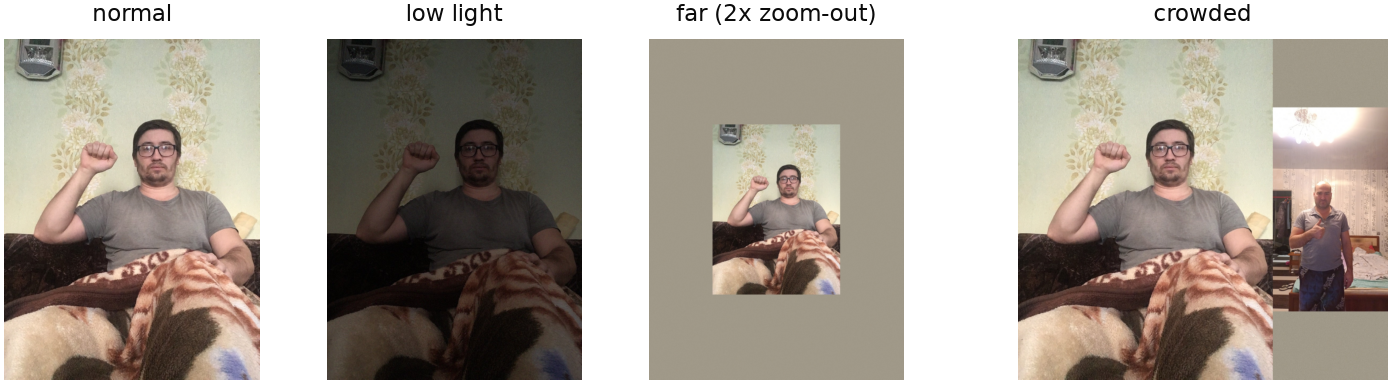
\includegraphics[width=\linewidth]{figures/conditions.png}
  \vspace{-1.5mm}
  \caption{One held-out subject in the four test conditions (crowded: another test subject added at 0.6$\times$).}
  \label{fig:cond}
  \vspace{-3mm}
\end{figure}
